 \documentclass[11pt]{article}
\usepackage[english]{babel}
\usepackage[utf8]{inputenc}
\usepackage[margin=0.5in]{geometry}
\usepackage{amsmath}
\usepackage{amsthm}
\usepackage{amsfonts}
\usepackage{amssymb}
\usepackage[usenames,dvipsnames]{xcolor}
\usepackage{graphicx}
\usepackage[siunitx]{circuitikz}
\usepackage{tikz}
\usepackage{tkz-berge}
\usetikzlibrary{positioning, automata, backgrounds}
\usepackage[colorinlistoftodos, color=orange!50]{todonotes}
\usepackage{hyperref}
\usepackage[numbers, square]{natbib}
\usepackage{fancybox}
\usepackage{epsfig}
\usepackage{soul}
\usepackage[framemethod=tikz]{mdframed}
\usepackage[shortlabels]{enumitem}
\usepackage[version=4]{mhchem}
\usepackage{multicol}
\usepackage{forest}
\usepackage{mathtools}
\usepackage{comment}
\usepackage{enumitem}
\usepackage[utf8]{inputenc}
\usepackage{listings}
\usepackage{color}
\usepackage[numbers]{natbib}
\usepackage{subfiles}
\usepackage{tkz-berge}
\usepackage{algorithm}
\usepackage[noend]{algpseudocode}
\usepackage{colortbl}


\newtheorem{prop}{Proposition}[section]
\newtheorem{thm}{Theorem}[section]
\newtheorem{lemma}{Lemma}[section]
\newtheorem{cor}{Corollary}[prop]

\theoremstyle{definition}
\newtheorem{definition}{Definition}

\theoremstyle{definition}
\newtheorem{required}{Problem}

\theoremstyle{definition}
\newtheorem{ex}{Example}

\newcommand{\interval}[4]{\draw (#2, #1) -- (#3, #1); % Usage: \interval{height}{start}{end}{label}
\draw (#2, #1-0.11) -- (#2, #1+0.11); % draw left whisker
\draw (#3, #1-0.11) -- (#3, #1+0.11); % draw right whisker
\node[] at (#2-0.25, #1) {#4};
}


\setlength{\marginparwidth}{3.4cm}
%#########################################################

%To use symbols for footnotes
\renewcommand*{\thefootnote}{\fnsymbol{footnote}}
%To change footnotes back to numbers uncomment the following line
%\renewcommand*{\thefootnote}{\arabic{footnote}}

% Enable this command to adjust line spacing for inline math equations.
% \everymath{\displaystyle}

% _______ _____ _______ _      ______ 
%|__   __|_   _|__   __| |    |  ____|
%   | |    | |    | |  | |    | |__   
%   | |    | |    | |  | |    |  __|  
%   | |   _| |_   | |  | |____| |____ 
%   |_|  |_____|  |_|  |______|______|
%%%%%%%%%%%%%%%%%%%%%%%%%%%%%%%%%%%%%%%

\title{
\normalfont \normalsize 
\textsc{CSCI 3104 Spring 2022 \\ 
Instructors: Profs. Chen and Layer} \\
[10pt] 
\rule{\linewidth}{0.5pt} \\[6pt] 
\huge Problem Set 7\\
\rule{\linewidth}{2pt}  \\[10pt]
}
%\author{Your Name}
\date{}

\begin{document}
\definecolor {processblue}{cmyk}{0.96,0,0,0}
\maketitle


%%%%%%%%%%%%%%%%%%%%%%%%%
%%%%%%%%%%%%%%%%%%%%%%%%%%
%%%%%%%%%%FILL IN YOUR NAME%%%%%%%
%%%%%%%%%%AND STUDENT ID%%%%%%%%
%%%%%%%%%%%%%%%%%%%%%%%%%%
\noindent
Due Date \dotfill March 15 \\
Name \dotfill \textbf{Julia Troni} \\
Student ID \dotfill \textbf{109280095} \\
Collaborators \dotfill \textbf{List Your Collaborators Here}

\tableofcontents

\section{Instructions}
{\small
 \begin{itemize}
	\item The solutions \textbf{must be typed}, using proper mathematical notation. We cannot accept hand-written solutions. \href{http://ece.uprm.edu/~caceros/latex/introduction.pdf}{Here's a short intro to \LaTeX.}
	\item You should submit your work through the \textbf{class Canvas page} only. Please submit one PDF file, compiled using this \LaTeX \ template.
	\item You may not need a full page for your solutions; pagebreaks are there to help Gradescope automatically find where each problem is. Even if you do not attempt every problem, please submit this document with no fewer pages than the blank template (or Gradescope has issues with it).

	\item You are welcome and encouraged to collaborate with your classmates, as well as consult outside resources. You must \textbf{cite your sources in this document.} \textbf{Copying from any source is an Honor Code violation. Furthermore, all submissions must be in your own words and reflect your understanding of the material.} If there is any confusion about this policy, it is your responsibility to clarify before the due date. 

	\item Posting to \textbf{any} service including, but not limited to Chegg, Reddit, StackExchange, etc., for help on an assignment is a violation of the Honor Code.

\end{itemize}}


\newpage
\section{Standard 19 - Dynamic Programming: Identify the Precise Subproblems}

\noindent The goal of this standard is to practice identifying the recursive structure. To be clear, you are \textbf{not} being asked for a precise mathematical recurrence. Rather, you are being asked to clearly and precisely identify the cases to consider. Identifying the cases can sometimes provide enough information to design a dynamic programming solution.

\subsection{Problem \ref{DP1}}
\begin{required} \label{DP1}
Consider the \textsf{Stair Climbing} problem, defined as follows.
\begin{itemize}
\item \textsf{Instance:} Suppose we have $n$ stairs, labeled $s_{1}, \ldots, s_{n}$. Associated with each stair $s_{k}$ is a number $a_{k} \geq 1$. At stair $s_{k}$, we may jump forward $i$ stairs, where $i \in \{ 1, 2, \ldots, a_{k}\}$. You start on $s_{1}$.

\item \textsf{Solution:} The number of ways to to reach $s_{n}$ from $s_{1}$.
\end{itemize}

\noindent \\ \textbf{Your job} is to clearly identify the recursive structure. That is, suppose we are solving the subproblem at stair $s_{k}$. What precise sub-problems do we need to consider?
\end{required}

\begin{proof}[Answer]
%Your answer

\begin{itemize}
\item First we will consider if $k=1$. The number of ways to reach $s_1$ from $s_1$ is trivially 0.
\item Next we consider if k=2. There is only 1 way to reach $s_2$ from $s_1$.
\item Then there is the case if $k>2$. Here, a person may jump forward any amount of stairs, that is they can hop $1, 2, \ldots, a_{k}$ stairs . Thus, we must consider the number of ways to reach $s_1 \rightarrow s_{k-1}$. And the number of ways to reach $s_{k-1}$ depend on the number of ways to reach $s_{k-2}$. In particular the number of ways to reach $s_{k-1}$ is all the ways to reach $s_{k-2}$+1, where the extra plus 1 is the hop directly from $s_{k-2}$ to $s_{1}$. 
\end{itemize}
\end{proof}



\newpage
\subsection{Problem \ref{DP2}}
\begin{required} \label{DP2}
Fix $n \in \mathbb{N}$. The \textit{Trust Game} on $n$ rounds is a two-player dynamic game. Here, Player I starts with \$100. The game proceeds as follows.
\begin{itemize}
\item \textbf{Round 1:} Player I takes a fraction of the \$100 (which could be nothing) to give to Player II. The money Player I gives to Player II is multiplied by 1.5 before Player II receives it. Player I keeps the remainder. (So for example, if Player I gives \$20 to Player II, then Player II receives \$30 and Player I is left with \$80).

\item \textbf{Round 2:} Player II can choose a fraction of the money they received to offer to Player I. The money offered to Player I increases by a multiple of $1.5$  before Player I receives it. Player II keeps the remainder.
\end{itemize}

\noindent \\ More generally, at round $i$, the Player at the current round (Player I if $i$ is odd, and Player II if $i$ is even) takes a fraction of the money in the current pile to send to the other Player and keeps the rest. That money increases by a factor of $1.5$ before the other player receives it. The game terminates if the current player does not send any money to the other player, or if round $n$ is reached. At round $n$, the money in the pile is split evenly between the two players. \\

\noindent Each individual player wishes to maximize the total amount of money they receive. \\

\noindent \textbf{Your job} is to clearly identify the recursive structure. That is, at round $i$, what precise sub-problems does the current player need to consider? [\textbf{Hint:} Do we have a smaller instance of the Trust Game after each round?]
\end{required}

\begin{proof}[Answer]
%Your answer
\begin{itemize}
\item Case 1: The player keeps all of the money in the current pile. In this case, the game would end, so the player would miss out on the possibility of earning more money, because the key idea is that every exchange increases the pile of money by 1.5. 
\item Case 2: The player gives all of the money in the current pile to the other player. In this case that recieving player would hence receive the maximum amount of money possible since 100\% of the pile will be multiplied by 1.5. At this point we will have a smaller instance of the trust game, where n is decreased by 1 round, because the player have the choice of what to do with the money: keep all, give all, or give some.
\item Case 3: The player keeps a fraction and gives a fraction. In this case, the amount of money in the pile will increase because the "gifted" amount of money will increase by 1.5. And, again have a smaller instance of the trust game, where n is decreased by 1 round, because the receiving player will choose among one of the 3 cases. 
\end{itemize}
\end{proof}




\newpage
\section{Standard 20- Dynamic Programming: Write Down Recurrences}

\subsection{Problem \ref{DP3}}

\begin{required} \label{DP3}
Suppose we have an $m$-letter alphabet $\Sigma = \{0, 1, \ldots, m-1\}$. Let $W_{n}$ be the set of strings $\omega \in \Sigma^{n}$ such that $\omega$ does not have $00$ as a substring. Let $f_{n} := |W_{n}|$. Write down an explicit recurrence for $f_{n}$, including the base cases. Clearly justify each recursive term.
\end{required}

\begin{proof}[Answer]
%Your answer here.

The first step is to write down the initial conditions: \\
Observe that $W_0 = {\emptyset}$, which is the string of length 0. So, $f_0 = 1$. \\
$W_1 = \{0,1,2, ... , m-1\}$, so  $f_1 = m$ \\

Now consider a string with  $w \in W_{n}$  of length $n \geq 2$. The first character $w_0 \in  \{0,1,2, ... , m-1\}$ \\
Now we have the following cases:
\begin{itemize}
\item Case 1: If $w_1 = 0$ then $w_2 \in  \{1,2, ... , m-1\}$, otherwise we would have the 00 substring. There are m-1 options for $w_2$ so we have $w= 0\cdot (m-1) \tau$ where $\tau \in W_{n-2}$. Thus there are $|W_{n-2}| = f_{n-2}$ string of the form $ 0\cdot (m-1) \tau$ in $W_n$
\item Case 2: If $w_1 \neq 0 $ that is $w_1 \in  \{1,2, ... , m-1\}$, then $w_2$ can be any character in $\sigma$. In this case, $w=(m-1)\cdot \tau$ where  $\tau \in W_{n-1}$, so we have $f_{n-1}$ ways to select $w$ in this case
\end{itemize}

So we have \\
$f_n= f_{n-2}+f_{n-1}$ with the initial conditions of  $f_0 = 1$ and $f_1 = m$ 

\end{proof}

%You may find the following commented code helpful in rendering a recurrence
\begin{comment}
\begin{align*}
f_{n} &= \begin{cases} \text{Case1} & : \text{Condition1}, \\ 
\text{Case2} & : \text{Condition2}. 
\end{cases}
\end{align*}
\end{comment}




\newpage
\subsection{Problem \ref{DP4}}

\begin{required} \label{DP4}
Suppose we have the alphabet $\Sigma = \{x, y\}$. For $n \geq 0$, let $W_{n}$ be the set of strings $\omega \in \{x, y\}^{n}$ where $\omega$ contains $yyy$ as a substring. Let $f_{n} := |W_{n}|$. Write down an explicit recurrence for $f_{n}$, including the base cases. Clearly justify each recursive term.
\end{required}

\begin{proof}[Answer]
%Your answer here.
If $n<3$, then we cannot have $yyy$ substring, so there are 0 options for this.\\
If n=3, then there is only 1 possibility for the substring $yyy$. \\

Now consider a string with  $w \in W_{n}$  of length $n> 3$.\\
Now we have the following cases:
\begin{itemize}
\item Case 1: If $w_0 \neq y$ then we will simply move on to check the rest of the string which is $w_1$ to $w_n$ so there is $f_{n-1}$ ways to construct the rest of the string. So we have $1\cdot f_{n-1}$
\item Case 2: If $w_0 = y $ and $w_1 \neq y$, then we examine $w_2$ to $w_n$ and there are $1\cdot1\cdot f_{n-2}$ ways to construct the string 
\item Case 3: If $w_0 =y$ and $w_1=y$, and $w_2 \neq y$, then there are $1\cdot1\cdot1\cdot f_{n-3}$ ways to construct the rest of the string. 
\item Case 4: Lastly, if $w_0 = y $ and $w_1 = y$ and $w_2=y$. Now we have the $yyy$ substring, so we have $2^{n-3}$
\end{itemize}

Thus we have \\
\begin{align*}
f_{n} &= \begin{cases} \text{0} & : \text{$n<3$}, \\ 
 \text{1} & : \text{n=3}, \\ 
\text{$ f_{n-3}+f_{n-2}+f_{n-1}+ 2^{n-3}$} & : \text{$n>3$}. 
\end{cases}
\end{align*}

\end{proof}




\newpage
\section{Standard 21- Dynamic Programming: Using Recurrences to Solve}

\subsection{Problem \ref{Recurrence1}}
\begin{required} \label{Recurrence1}
Given the following directed acyclic graph. Use dynamic programming to fill in a \textbf{one-dimensional} lookup table that counts number of paths from each node $j$ to 14, for $j \geq 1$. Note that a single vertex is considered a path of length $0$. \textbf{Fill in the lookup table for all vertices 1-14; and in addition, clearly show work for vertices 9-14}.

        % ----- FIGURE -----
        \begin{figure}[h!]
        \begin{center}
        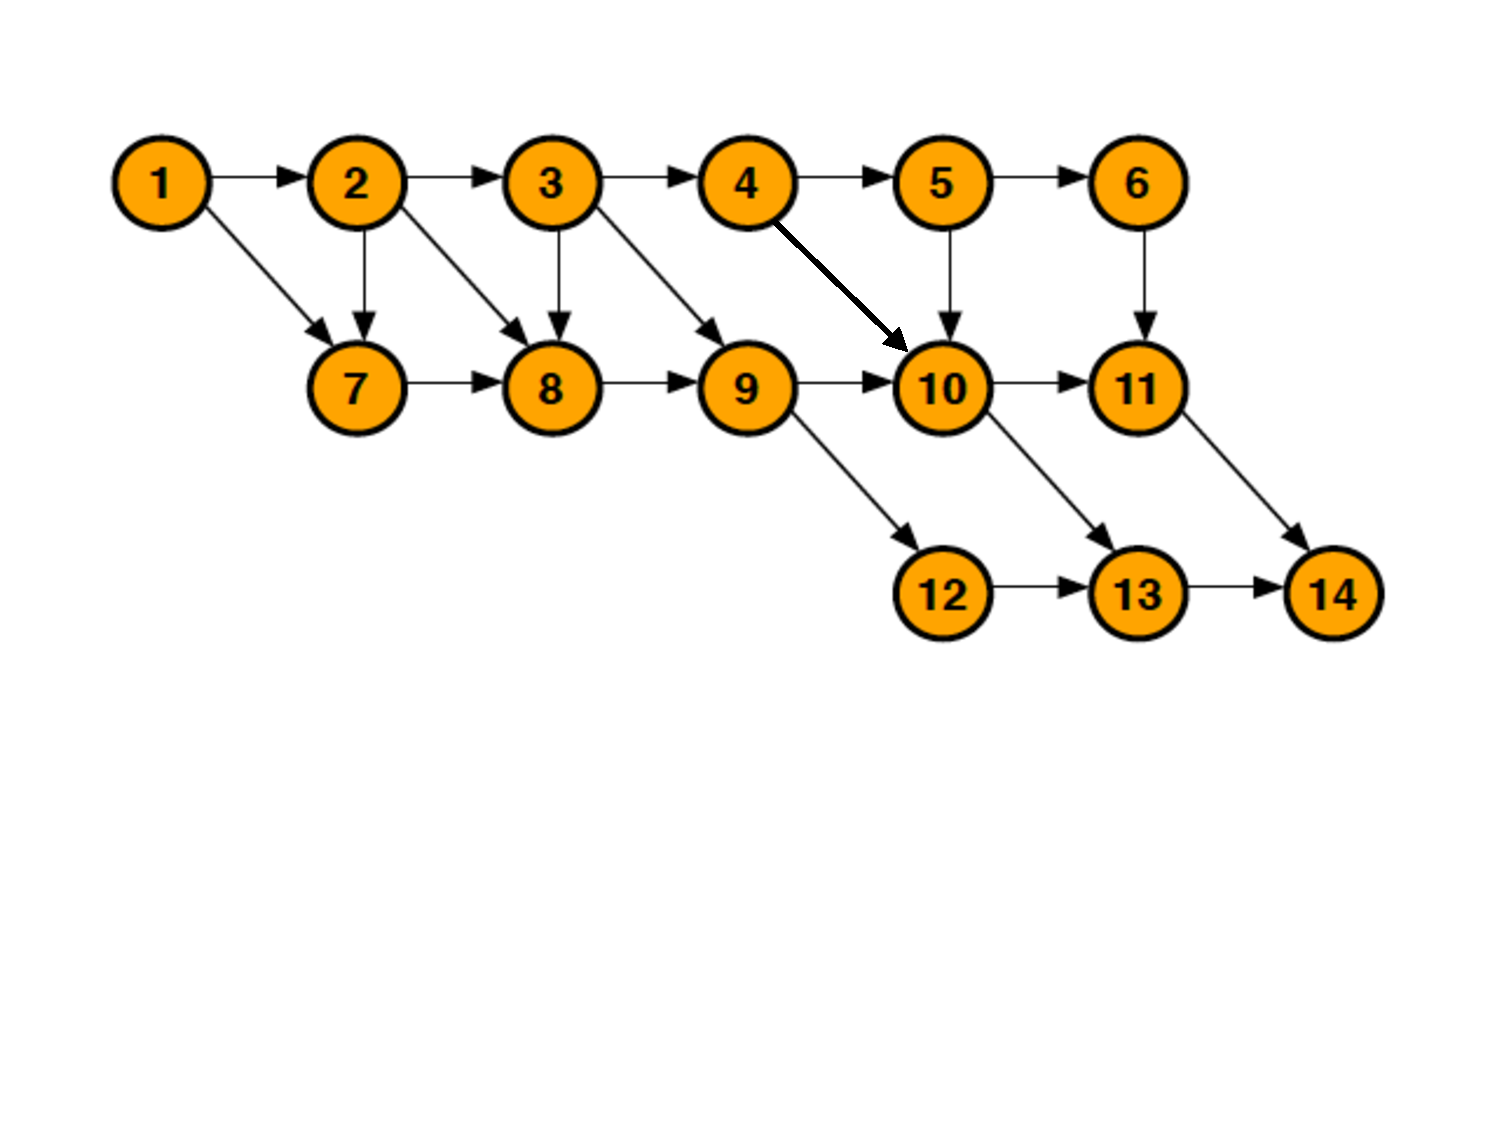
\includegraphics[scale=0.45]{dag_ps10.pdf} 
        \end{center}
        \end{figure}
        % ----------

\end{required}


\begin{proof}[Answer]
%Your answer

\centering
\begin{tabular}{|l|l|l|l|l|l|l|l|l|l|l|l|l|l|l|} 
\hline
\rowcolor[rgb]{0.753,0.753,0.753} Node              & 1  & 2  & 3  & 4 & 5 & 6 & 7 & 8 & 9 & 10 & 11 & 12 & 13 & 14  \\ 
\hline
{\cellcolor[rgb]{0.753,0.753,0.753}}Number of Paths & 20 & 17 & 11 & 5 & 3 & 1 & 3 & 3 & 3 & 2  & 1  & 1  & 1  & 1   \\
\hline
\end{tabular}

We begin at node 14:
\begin{itemize}
\item When j=14 this is a single vertex and hence path length is 0, so number of paths from vertex 14 to 14 is 0.
\item When j=13 there is only 1 path from 13 to 14, so number of paths from vertex 13 to 14 is 1.
\item When j=12 there is only 1 outgoing edge. So, that means there is only 1 route to leave vertex 12. So we take the number of paths of its neighbor. This is (number of paths from 13 to 14)=1, so number of paths from vertex 12 to 14 is 1.
\item When j=11 there is also only 1 outgoing edge, which is to vertex 14, so that means there is only 1 route to vertex 14. So number of paths from vertex 11 to 14 is 1.
\item When j=10 there are 2 outgoing edges. So, we must consider that there are 2 options to get to vertex 14. So we take the number of paths of each of its neighbors, 11 and 13. This is (number of paths from 11 to 14) + (number of paths from 13 to 14)=1+1, so number of paths from vertex 10 to 14 is 2.
\item When j=9 there are also 2 outgoing edges. So, we must consider that there are 2 options to get to vertex 14. So we take the number of paths of each of its neighbors, 10 and 12. This is (number of paths from 10 to 14) + (number of paths from 12 to 14)=2+1, so number of paths from vertex 9 to 14 is 3.
\end{itemize}
\end{proof}




\newpage
\subsection{Problem \ref{Recurrence2}}
\begin{required} \label{Recurrence2}
Consider the following input for the Knapsack problem with a capacity $W=12$:\\

 \begin{tabular}{r|c|c|c|c|c|c}
        item $i$  & 1  & 2 &3 &4 &5 &6 \\
                \hline
        value $v_i$ &2 & 7& 18&23 &29 &35 \\
          \hline
        weight $w_i$ & 1 & 2  & 5& 6& 7& 9\\
                 \end{tabular}

\vspace{1mm}
\noindent \\ 
Fill in a lookup table, similar to the example on page 12 of course notes for week 9 (see Week 9 under ``Modules" of the course canvas). In addition, clearly explain how you obtain the maximum values/profits $OPT(6, w)$, $w=7,~8,~9,~10,~11,~12$.

\end{required}

\begin{proof}[Answer]
%Your answer here

The lookup table is below \\

\centering
\begin{tabular}{|l|l|l|l|l|l|l|l|l|l|l|l|l|l|} 
\hline
\rowcolor[rgb]{0.753,0.753,0.753}                  & 0 & 1 & 2 & 3 & 4 & 5  & 6  & 7  & 8  & 9  & 10 & 11 & 12  \\ 
\hline
{\cellcolor[rgb]{0.753,0.753,0.753}}i=0            & 0 & 0 & 0 & 0 & 0 & 0  & 0  & 0  & 0  & 0  & 0  & 0  & 0   \\ 
\hline
{\cellcolor[rgb]{0.753,0.753,0.753}}i=1, v=2, w=1  & 0 & 2 & 2 & 2 & 2 & 2  & 2  & 2  & 2  & 2  & 2  & 2  & 2   \\ 
\hline
{\cellcolor[rgb]{0.753,0.753,0.753}}i=2, v=7, w=2  & 0 & 2 & 7 & 9 & 9 & 9  & 9  & 9  & 9  & 9  & 9  & 9  & 9   \\ 
\hline
{\cellcolor[rgb]{0.753,0.753,0.753}}i=3, v=18, w=5 & 0 & 2 & 7 & 9 & 9 & 18 & 20 & 25 & 27 & 27 & 27 & 27 & 27  \\ 
\hline
{\cellcolor[rgb]{0.753,0.753,0.753}}i=4, v=23, w=6 & 0 & 2 & 7 & 9 & 9 & 18 & 23 & 25 & 30 & 32 & 32 & 41 & 43  \\ 
\hline
{\cellcolor[rgb]{0.753,0.753,0.753}}i=5, v=29, w=7 & 0 & 2 & 7 & 9 & 9 & 18 & 23 & 29 & 31 & 36 & 38 & 41 & 47  \\ 
\hline
{\cellcolor[rgb]{0.753,0.753,0.753}}i=6, v=35, w=9 & 0 & 2 & 7 & 9 & 9 & 18 & 23 & 29 & 31 & 36 & 38 & 42 & 47  \\
\hline
\end{tabular}


\begin{itemize}
\item To obtain $OPT(6, 7)$ we will apply the case when  $w_i>w$ because $9>7$. \\ So, $OPT(i-1,w)=OPT(5,7)=29$ so $OPT(5,7)= 29$
\item To obtain $OPT(6, 8)$ we will also apply the case when  $w_i>w$ because $9>8$. \\ So, $OPT(i-1,w)=OPT(5,8)=31$ so $OPT(5,8)= 31$\\
\end{itemize}
To obtain $OPT(6, w)$  for w= 8,9,10,11,12 we will apply the case when  $w_i<=w$, which is $max\{OPT(i-1,w), v_i+OPT(i-1,w-w_i)\}$.
\begin{itemize}
\item For $OPT(6, 9)$, we have \\ $max\{OPT(5,9), 35+OPT(5,0)\}= max\{36, 35+0\}=max\{36,35\}= 36$. \\So,  $OPT(6, 9)= 36$ 
\item For $OPT(6, 10)$, we have \\ $max\{OPT(5,10), 35+OPT(5,1)\}= max\{38, 35+2\}=max\{38,37\}= 38$. \\So,  $OPT(6, 10)= 38$ 
\item For $OPT(6, 11)$, we have \\ $max\{OPT(5,11), 35+OPT(5,2)\}= max\{41, 35+7\}=max\{41,42\}= 42$. \\So,  $OPT(6, 11)= 42$ 
\item For $OPT(6, 12)$, we have \\ $max\{OPT(5,12), 35+OPT(5,3)\}= max\{47, 35+9\}=max\{47,44\}= 47$. \\So,  $OPT(6, 12)= 47$ 
\end{itemize}

\end{proof}

\end{document} % NOTHING AFTER THIS LINE IS PART OF THE DOCUMENT



